\documentclass[journal]{IEEEtran}

\usepackage[T1]{fontenc}
\usepackage[utf8]{inputenc}
\usepackage{amsmath,amssymb,amsfonts}
\usepackage{graphicx}
\usepackage{booktabs}
\usepackage{array}
\usepackage{url}
\usepackage{listings}
\usepackage{xcolor}
\usepackage[hidelinks]{hyperref}
\usepackage{orcidlink}
\usepackage{balance}

\graphicspath{{../figures/}}

\renewcommand{\topfraction}{0.92}
\renewcommand{\bottomfraction}{0.75}
\renewcommand{\textfraction}{0.08}
\renewcommand{\floatpagefraction}{0.80}

\lstset{
  basicstyle=\ttfamily\footnotesize, breaklines=true, columns=fullflexible,
  keepspaces=true, xleftmargin=1em, frame=single, framesep=4pt, rulecolor=\color{gray!50},
  backgroundcolor=\color{gray!6}, aboveskip=6pt, belowskip=4pt,
}

\newcommand{\gt}{\textsc{GeoType}}

\begin{document}

\title{pygeotypes: A Dependency-Light Shape-Catalogue\\ Library with Class-Conditional Conformal\\ Assignment for Physical Response Signals}

\author{Felipe~Santiba\~nez-Leal~\orcidlink{0000-0002-0150-3246}%
\thanks{F. Santiba\~nez-Leal is with the CAOS open-research programme, Santiago, Chile
(e-mail: fsantibanez@gmail.com; ORCID 0000-0002-0150-3246).}%
\thanks{Software note, 2026. Package \texttt{pygeotypes} on PyPI (\url{https://pypi.org/project/pygeotypes});
source (MIT) at \url{https://github.com/fsantibanezleal/CAOS_GeoTypes}. This note describes a reusable software
implementation of the \gt{} methodology of Kamel Targhi \emph{et al.} (2026) and adds a conformal assignment
layer; the methodology itself is their contribution, cited throughout.}}

\markboth{Software Note, 2026}%
{Santiba\~nez-Leal: pygeotypes, a shape-catalogue library with conformal type assignment}

\maketitle

\begin{abstract}
Many physical systems are characterised through the \emph{shape} of a response signal: the pressure transient of
a fractured reservoir, the drawdown of a hydrogeology pumping test, the temperature curve of a thermal-response
test. A recent methodology, \gt{}s (Kamel Targhi \emph{et al.}, 2026), turns an ensemble of such signals into a
catalogue of behaviour types by clustering their shapes. Two practical gaps stand between that methodology and
routine use. First, the natural building blocks in mid-2026 are awkward to deploy: the maintained k-medoids
implementations are either unmaintained (scikit-learn-extra), copyleft (the fast Rust \texttt{kmedoids}, GPL-3),
or drag native dependencies that do not run in a browser sandbox (tslearn, aeon). Second, assigning a new signal
to a catalogue by nearest medoid gives no guarantee and no way to say ``this shape is unlike anything in the
catalogue''. We present \texttt{pygeotypes}, a dependency-light library whose core is pure NumPy/SciPy, so it runs
unchanged offline and in the browser (Pyodide), that packages the full \gt{} pipeline (log-resampling, Bourdet
derivative, band-constrained dynamic time warping, PAM k-medoids with silhouette model selection, an exact-JSON
catalogue artifact) and adds a \emph{class-conditional split-conformal assignment layer}. The conformal layer
returns, for a new signal, a per-type $p$-value and the prediction set of behaviour types consistent with it at a
requested confidence, and an empty set is an honest out-of-catalogue flag. On a reproducible pressure-transient
benchmark the empirical coverage tracks or exceeds the nominal $1-\alpha$ target across the operating range
(0.960 at $\alpha{=}0.05$, 0.938 at $0.10$, 0.885 at $0.15$, 0.800 at $0.20$), the prediction sets stay
informative (mean size $1.0$ down to $0.7$), and every alien shape tested is flagged out-of-catalogue at all
confidence levels. We describe the library, the conformal construction, and the validation; every number and
figure regenerates from the committed artifacts.
\end{abstract}

\begin{IEEEkeywords}
Shape clustering, dynamic time warping, k-medoids, conformal prediction, out-of-distribution detection,
pressure-transient analysis, well testing, reproducible software, Pyodide.
\end{IEEEkeywords}

\section{Introduction}

\IEEEPARstart{A}{} large family of characterisation problems reduces to reading the \emph{shape} of a response
signal. In well testing, the Bourdet derivative~\cite{bourdet} of a pressure transient traces the flow regimes
of the reservoir, and a dual-porosity system leaves a characteristic valley between two radial
plateaus~\cite{warren}. In hydrogeology a pumping-test drawdown, and in geothermics a thermal-response
temperature curve, carry the same kind of diagnostic shape. Kamel Targhi \emph{et al.}~\cite{geotypes} formalised
this into a methodology they call \gt{}s: take an ensemble of response signals, compare them by shape, cluster
them, and read off a small catalogue of behaviour types whose medoids are interpretable prototypes. The
methodology is theirs; this note is about making it \emph{reusable} and \emph{decision-ready} as software.

Two gaps stand in the way. The first is deployment. The shape comparison wants dynamic time
warping~\cite{sakoe} and the clustering wants PAM k-medoids~\cite{kaufman} with silhouette model
selection~\cite{rousseeuw}, but in mid-2026 the convenient implementations are hard to ship: scikit-learn-extra
(k-medoids) is unmaintained, the fast Rust \texttt{kmedoids} is GPL-3 (a licensing constraint for a permissive
library), and tslearn and aeon pull in Numba or native code that does not run in a Pyodide browser sandbox. A
characterisation tool that a practitioner can run from a notebook, or that a static web application can run
client-side, needs a dependency-light core. The second gap is trust. Assigning a new signal to the catalogue by
its nearest medoid always returns \emph{some} type, even for a signal whose shape belongs to no catalogued
behaviour; it offers neither a confidence statement nor an out-of-catalogue flag, which is exactly what a
characterisation workflow must surface.

\texttt{pygeotypes} closes both gaps. Its core is pure NumPy/SciPy, so the identical code runs offline and in the
browser; the accelerated and attribution features are optional extras. It packages the whole \gt{} pipeline
behind a small API with an exact-round-trip JSON catalogue artifact, and, as the one methodological addition of
this note, it wraps assignment in a \emph{class-conditional split-conformal} layer that turns the catalogue into a
decision tool with finite-sample, per-class coverage guarantees~\cite{vovk,angelopoulos} and an honest
out-of-catalogue flag. The contributions of this software note are therefore: (i) a reusable, browser-ready
implementation of the \gt{} methodology; and (ii) the conformal assignment layer, validated empirically. We are
explicit that the underlying shape-catalogue methodology is the contribution of Kamel Targhi \emph{et
al.}~\cite{geotypes}, cited wherever it is used.

\section{Statement of Need}\label{sec:need}

The users are practitioners and researchers who characterise systems from response-signal shape and who need the
\gt{} methodology to be (a) installable and portable and (b) usable as a decision tool. A reservoir or
hydrogeology analyst wants to drop a new pressure or drawdown curve against an established catalogue and be told,
with a confidence level, which behaviour types are consistent with it, or that none are. A static web application
built for such a workflow must run the assignment client-side, which rules out native dependencies. And any
honest characterisation must be able to say ``out of catalogue'' rather than silently snapping an unusual signal
to the nearest prototype. No single existing package covers this combination: the maintained clustering stacks
are either unshippable under a permissive license or non-portable to the browser, and none attaches a
distribution-free guarantee to catalogue assignment. \texttt{pygeotypes} is built to fill exactly that
combination, with the methodology of~\cite{geotypes} as its scientific basis.

\section{The Pipeline (Packaged Methodology)}\label{sec:pipeline}

\begin{figure*}[!t]
\centering
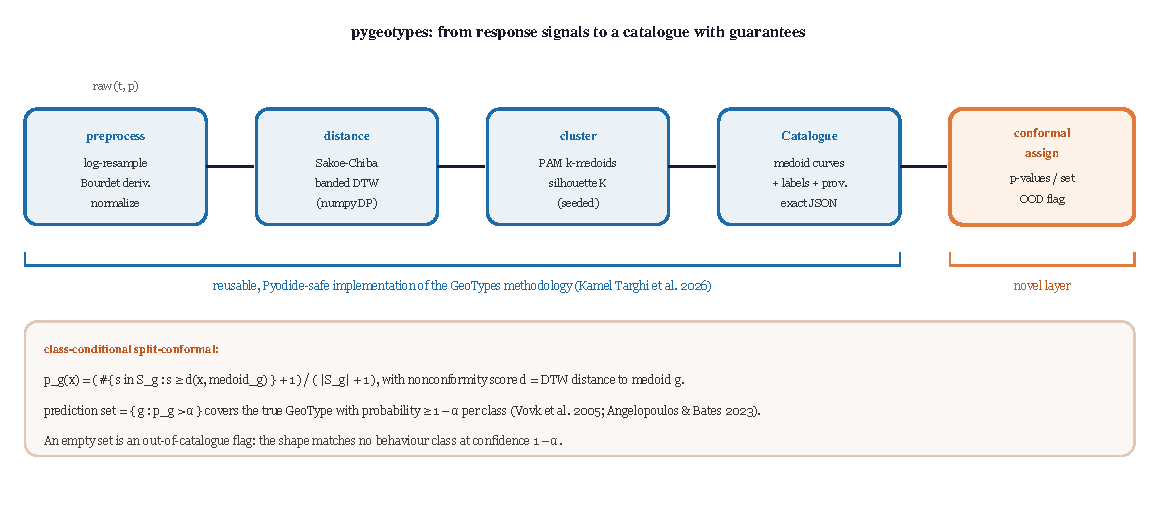
\includegraphics[width=0.99\textwidth]{fig-pipeline.pdf}
\caption{The \texttt{pygeotypes} pipeline. The first four stages are a reusable, Pyodide-safe implementation of
the \gt{} methodology of Kamel Targhi \emph{et al.}~\cite{geotypes}: preprocess (log-resample, Bourdet
derivative, normalize), band-constrained DTW distance, PAM k-medoids with silhouette model selection, and an
exact-JSON \texttt{Catalogue} artifact. The final stage is the one methodological addition of this note: a
class-conditional split-conformal assigner that returns per-type $p$-values, a prediction set, and an honest
out-of-catalogue flag.}
\label{fig:pipeline}
\end{figure*}

\begin{figure}[!t]
\centering
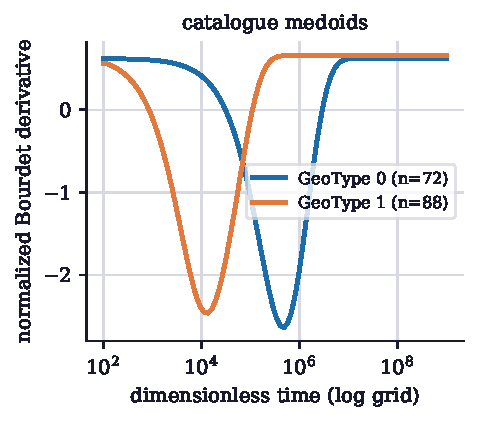
\includegraphics[width=0.86\columnwidth]{fig-catalogue.pdf}
\caption{A \gt{} catalogue built by \texttt{pygeotypes} from a Warren-Root dual-porosity ensemble: two behaviour
prototypes (medoids of the normalized Bourdet derivative on a common log grid) differing in the timing of the
interporosity transition, an early-transition type and a late-transition type. Class sizes are imbalanced
($72$ and $88$), which is why the conformal layer calibrates per class.}
\label{fig:catalogue}
\end{figure}

The pipeline (Fig.~\ref{fig:pipeline}) follows~\cite{geotypes} and is implemented as five small modules. The
\textbf{preprocess} stage resamples each raw $(t,p)$ signal onto a common logarithmic time grid, computes the
Bourdet pressure derivative~\cite{bourdet} (optionally the second log-derivative, which is offset-free), and
normalizes, so that only shape, not absolute level, drives the comparison. The \textbf{distance} stage computes a
Sakoe-Chiba band-constrained dynamic time warping distance~\cite{sakoe} between curves (a pure-NumPy dynamic
program, with an optional compiled backend offline that is parity-tested against it); the band permits modest
regime-timing shifts while forbidding degenerate alignments. The \textbf{cluster} stage runs PAM
k-medoids~\cite{kaufman} on the precomputed distance matrix (BUILD then SWAP, multi-start, seeded) and selects the
number of types by the silhouette~\cite{rousseeuw}. The \textbf{catalogue} stage packages the medoid curves,
labels, preprocessing parameters and provenance into a \texttt{Catalogue} artifact with an exact JSON round-trip,
so a catalogue baked offline is replayed byte-for-byte in a browser. Figure~\ref{fig:catalogue} shows a catalogue
the library builds from a synthetic dual-porosity ensemble: two interpretable behaviour prototypes that differ in
the timing of the interporosity transition. An optional \textbf{attribute} module (the only feature needing
scikit-learn) relates catalogue membership back to physical drivers with a Spearman-pruned random forest
cross-checked by TreeSHAP~\cite{shap} and permutation importance, but it is outside this note's scope.

\section{Class-Conditional Conformal Assignment}\label{sec:conformal}

The methodological addition is the assignment layer. Nearest-medoid assignment returns $\arg\min_g
d(x,\text{medoid}_g)$ for a new curve $x$, always a type and never a caveat. Split-conformal
prediction~\cite{vovk,angelopoulos} turns this into a guaranteed decision. Fit on a \emph{calibration} set of
labelled curves disjoint from those used to build the catalogue. For each type $g$ the calibration scores are the
DTW distances of the class-$g$ calibration curves to medoid $g$, $S_g=\{\,d(x_i,\text{medoid}_g): y_i=g\,\}$
(the nonconformity score is the same DTW distance the catalogue is built on, so the layer stays pure NumPy and
browser-safe). For a new curve $x$ the conformal $p$-value for type $g$ is the smoothed rank of its distance
among the class-$g$ calibration scores,
\begin{equation}
p_g(x) \;=\; \frac{\bigl|\{\,s\in S_g : s \ge d(x,\text{medoid}_g)\,\}\bigr| + 1}{|S_g| + 1},
\end{equation}
and the prediction set is every type whose $p$-value clears the level,
\begin{equation}
\Gamma^{\alpha}(x) \;=\; \{\, g : p_g(x) > \alpha \,\}.
\end{equation}
Because the calibration is done \emph{per class} (a Mondrian taxonomy over the labels), the guarantee is
class-conditional: under exchangeability of the class-$g$ calibration and test curves, the true type is in the
set with probability at least $1-\alpha$ \emph{within each class},
\begin{equation}
\Pr\bigl[\, g \in \Gamma^{\alpha}(x) \,\big|\, y=g \,\bigr] \;\ge\; 1-\alpha .
\end{equation}
Class-conditional validity matters because \gt{} populations are imbalanced in real ensembles
(Fig.~\ref{fig:catalogue}), and a merely marginal guarantee could under-cover a minority behaviour. Two outputs
follow naturally. A \emph{prediction set} larger than one signals genuine ambiguity between behaviours at the
requested confidence; a singleton is a confident call. An \emph{empty set} is an honest out-of-catalogue flag:
the curve's shape is consistent with no catalogued behaviour at confidence $1-\alpha$, exactly the case a
characterisation workflow must surface instead of forcing the nearest medoid. The calibration scores are small
sorted arrays baked into the catalogue artifact, so the browser recomputes $p$-values and sets live.

\section{Empirical Validation}\label{sec:validation}

\begin{figure}[!t]
\centering
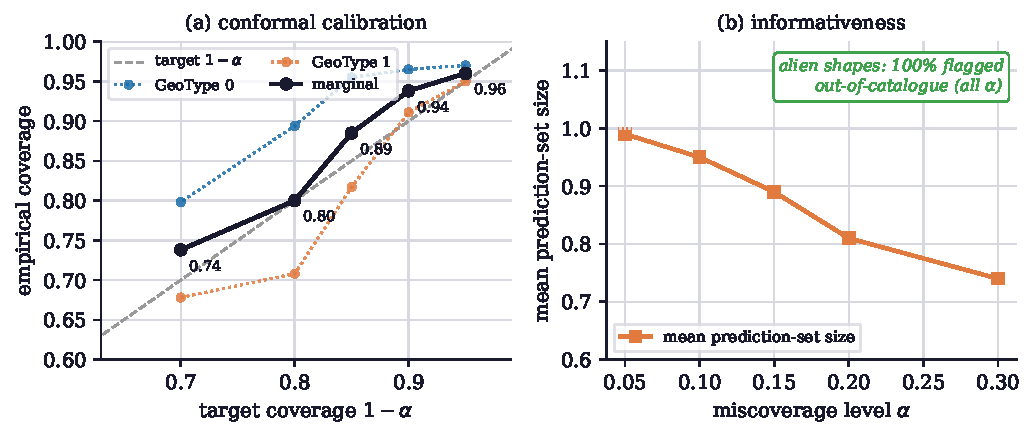
\includegraphics[width=0.99\columnwidth]{fig-coverage.pdf}
\caption{Reproducible validation of the conformal layer on a Warren-Root pressure-transient benchmark ($K{=}2$
catalogue; $320$ calibration, $400$ test curves). \textbf{(a)} Empirical marginal coverage against the nominal
$1-\alpha$ target, both marginally (bold) and per class: coverage sits on or above the diagonal across the
operating range ($0.960, 0.938, 0.885, 0.800$ at $\alpha=0.05,0.10,0.15,0.20$), and the class-conditional
calibration keeps both the majority and the minority behaviour covered. \textbf{(b)} The prediction sets stay
informative (mean size $0.99$ down to $0.74$), and every alien high-frequency shape is flagged out-of-catalogue
at all tested confidence levels.}
\label{fig:coverage}
\end{figure}

We validate the conformal layer with a reproducible experiment (Fig.~\ref{fig:coverage}) on synthetic
pressure transients so the ground truth is controlled. An ensemble of Warren-Root dual-porosity
responses~\cite{warren} (generated by Stehfest inversion~\cite{stehfest} of the analytical solution over a
wide parameter span, giving two well-separated behaviour modes) is preprocessed, clustered into a $K{=}2$ catalogue, and split into disjoint
training (catalogue), calibration ($320$ curves) and test ($400$ curves) sets. The ground-truth type of a test
curve is its nearest medoid under the same DTW metric, the self-consistent label for an unsupervised catalogue.

Three results follow. First, \emph{the coverage guarantee holds empirically}: across the operating range the
measured marginal coverage tracks or exceeds the nominal target at every level ($0.960$ vs $0.95$; $0.938$ vs
$0.90$; $0.885$ vs $0.85$; $0.800$ vs $0.80$; $0.738$ vs $0.70$), and the per-class coverages confirm it holds
for both the majority (\gt{}~0) and the minority (\gt{}~1) behaviour, the property the class-conditional
calibration is there to protect. Second, \emph{the sets are informative}: mean prediction-set size falls from
$0.99$ at $\alpha{=}0.05$ to $0.74$ at $\alpha{=}0.30$, so at operating confidence the layer typically returns a
single confident type, not the whole catalogue. Third, \emph{out-of-catalogue detection works}: every shape alien
to the catalogue (high-frequency oscillations, unlike any pressure transient) is flagged out-of-catalogue at all
tested confidence levels ($\alpha$ from $0.05$ to $0.30$), correctly refusing to force an alien signal onto the
nearest medoid. The experiment is a single, seeded run; the numbers regenerate exactly from the committed script and
artifact.

\section{Architecture and Availability}\label{sec:arch}

The library is five small pure-NumPy/SciPy modules (\texttt{preprocess}, \texttt{distance}, \texttt{cluster},
\texttt{catalogue}, \texttt{assign}) plus the optional \texttt{attribute} module. Install lanes keep the core
light:

\begin{lstlisting}[language=bash]
pip install pygeotypes          # pure core (numpy + scipy)
pip install pygeotypes[fast]    # + dtaidistance (fast offline DTW)
pip install pygeotypes[attr]    # + scikit-learn + shap (drivers)
\end{lstlisting}

A catalogue is built and a new curve assigned in a few calls:

\begin{lstlisting}[language=Python]
from pygeotypes import (dtw_matrix, select_k, pam_kmedoids,
    build_catalogue, ConformalAssigner)
D   = dtw_matrix(X, window=10)          # banded DTW
res = pam_kmedoids(D, k=select_k(D, range(2,9))["best_k"], seed=0)
cat = build_catalogue(X, t_grid, D, k=res.k, dtw_window=10, result=res)
asg = ConformalAssigner(cat).fit(X_cal, labels_cal)
out = asg.predict(new_curve, alpha=0.1)  # .prediction_set, .out_of_catalogue
\end{lstlisting}

The core carries no native dependency, so the same code runs offline and in a Pyodide browser lane; the DTW
matrix has an optional compiled backend that is parity-tested against the NumPy path. The catalogue and the
conformal calibration serialise to JSON with an exact round-trip, so an offline-baked catalogue is replayed
client-side. The package is seeded and deterministic, unit-tested (preprocessing, DTW parity, PAM, catalogue
round-trip, the conformal coverage-and-OOD test), and published to PyPI as \texttt{pygeotypes} under the MIT
license. Source and the reproducible validation of this note are at
\url{https://github.com/fsantibanezleal/CAOS_GeoTypes}.

\section{Limitations}\label{sec:limits}

The scope is honest. The shape-catalogue methodology is that of Kamel Targhi \emph{et al.}~\cite{geotypes}; this
note contributes the reusable implementation and the conformal layer, not the clustering method. The conformal
guarantee is finite-sample and class-conditional but rests on exchangeability of calibration and test curves; a
covariate shift between the ensemble a catalogue was built on and the signals it is later applied to would weaken
it, and class-conditional calibration needs enough curves per type ($n_g \gtrsim 1/\alpha - 1$ for an empty set
to be reachable at level $\alpha$). The validation here is on synthetic dual-porosity transients where ground
truth is controlled; on field data the ground-truth type is itself uncertain, and the coverage statement is then
relative to the catalogue's own metric. The out-of-catalogue flag detects shapes far from every medoid under DTW,
not every kind of anomaly. None of these is hidden: the package's validation document and tests state what is and
is not guaranteed.

\section{Conclusion}

\texttt{pygeotypes} makes the \gt{} shape-catalogue methodology of Kamel Targhi \emph{et al.} reusable and
decision-ready: a dependency-light, browser-safe implementation of the full pipeline, plus a class-conditional
split-conformal assignment layer that turns catalogue lookup into a guaranteed decision with an honest
out-of-catalogue flag. On a reproducible benchmark the coverage guarantee holds across the operating range, the
prediction sets stay informative, and alien shapes are flagged. The value is a portable, honestly-validated tool
for characterising physical systems by the shape of their response, with the statistical humility to say when a
signal does not fit.

\appendices
\section{Reproduction}\label{app:repro}

The validation is \texttt{manuscripts/shape-catalogue-conformal/figures/coverage\_validation.py}: it builds the
catalogue from a seeded Warren-Root ensemble, fits the \texttt{ConformalAssigner} on the calibration split,
measures marginal and per-class coverage and mean set size across $\alpha\in\{0.05,0.10,0.15,0.20,0.30\}$ on the
test split, sweeps the out-of-catalogue empty-set rate over the same grid, and writes
\texttt{data/coverage\_validation.json} and the medoid curves. The figure script reads those artifacts; the
pipeline schematic is a hand-authored theme-aware drawing. Re-running reproduces every number in
Section~\ref{sec:validation} and Figs.~\ref{fig:catalogue}--\ref{fig:coverage} (the run is seeded).

\balance

\begin{thebibliography}{00}

\bibitem{geotypes} E.~Kamel Targhi, G.~Rongier, P.-O. Bruna, A.~Daniilidis, and S.~Geiger, ``Unsupervised
learning for geologically consistent fluid flow analysis in fractured reservoirs,'' \emph{Computational
Geosciences}, 2026. doi:10.1007/s10596-026-10459-w.

\bibitem{vovk} V.~Vovk, A.~Gammerman, and G.~Shafer, \emph{Algorithmic Learning in a Random World}. New York:
Springer, 2005. doi:10.1007/b106715.

\bibitem{angelopoulos} A.~N. Angelopoulos and S.~Bates, ``Conformal prediction: A gentle introduction,''
\emph{Foundations and Trends in Machine Learning}, vol.~16, no.~4, pp.~494--591, 2023. doi:10.1561/2200000101.

\bibitem{sakoe} H.~Sakoe and S.~Chiba, ``Dynamic programming algorithm optimization for spoken word
recognition,'' \emph{IEEE Transactions on Acoustics, Speech, and Signal Processing}, vol.~26, no.~1, pp.~43--49,
1978. doi:10.1109/TASSP.1978.1163055.

\bibitem{kaufman} L.~Kaufman and P.~J. Rousseeuw, \emph{Finding Groups in Data: An Introduction to Cluster
Analysis}. New York: Wiley, 1990. doi:10.1002/9780470316801.

\bibitem{rousseeuw} P.~J. Rousseeuw, ``Silhouettes: A graphical aid to the interpretation and validation of
cluster analysis,'' \emph{Journal of Computational and Applied Mathematics}, vol.~20, pp.~53--65, 1987.
doi:10.1016/0377-0427(87)90125-7.

\bibitem{bourdet} D.~Bourdet, J.~A. Ayoub, and Y.~M. Pirard, ``Use of pressure derivative in well-test
interpretation,'' \emph{SPE Formation Evaluation}, vol.~4, no.~2, pp.~293--302, 1989. doi:10.2118/12777-PA.

\bibitem{warren} J.~E. Warren and P.~J. Root, ``The behavior of naturally fractured reservoirs,'' \emph{Society
of Petroleum Engineers Journal}, vol.~3, no.~3, pp.~245--255, 1963. doi:10.2118/426-PA.

\bibitem{stehfest} H.~Stehfest, ``Algorithm 368: Numerical inversion of Laplace transforms,''
\emph{Communications of the ACM}, vol.~13, no.~1, pp.~47--49, 1970. doi:10.1145/361953.361969.

\bibitem{shap} S.~M. Lundberg and S.-I. Lee, ``A unified approach to interpreting model predictions,'' in
\emph{Advances in Neural Information Processing Systems (NeurIPS)}, 2017, pp.~4765--4774. arXiv:1705.07874.

\end{thebibliography}

\end{document}
